\section{Gostota periodičnih točk}

Pravimo, da je periodična točka \(p\) s periodo \(n\) \emph{odbojna}, če je \(\abs{(f^n)' (p)} > 1\). Intuitivno to pomeni, da se vsaka točka, ki je blizu \(p\), od njene orbite ``oddalji''. Tako dokažemo močnejšo različico izreka o gostoti odbojnih točk.

\begin{izrek}[Gostota odbojnih periodičnih točk] \label{thm:periodicdense}
    Naj bo \(U \subset \CC\) neprazna in odprta množica. Potem obstaja odbojna periodična točka \(p \in U\).
\end{izrek}

\begin{lema}[Veje inverza preslikave \texorpdfstring{\(f^2\)}{f^2}] \label{lem:inversebranches}
    Naj bo \(z_0 \in \CC \setminus \set{0}\). Potem obstaja disk \(\triangle\) s središčem v \(z_0\) in število \(\rho \geq 0\) z naslednjo lastnostjo. Za vsak disk \(D\) z radijem \(2 \pi\) in središčem v točki z realnim delom vsaj \(\rho\), obstaja preslikava \(\phi \colon \triangle \to D\), za katero je \(f^2 \prt{\phi (z)} = z\) in \(|\phi' (z)| \leq 1\) za vsak \(z \in \triangle\).
\end{lema}

\noindent Lema nekoliko posploši trditev \ref{prop:lare_disks}. Poleg tega, da okrog \(z_0\) obstaja disk \(\triangle\), ki je v celoti vsebovan v \(f^2 (D)\), na \(\triangle\) lahko definiramo vejo preslikave \(f^{-2}\), ki slika v \(D\).

\begin{dokaz}
    Naj bo \(\varepsilon \coloneq \frac{|z_0|}{2}\) in \(\triangle \coloneq D_{\varepsilon} (z_0)\). Za vsak \(n \in \ZZ\) obstaja veja logaritma \(L_n\) na \(\triangle\), katere vrednosti imajo imaginarne dele med \(\Arg (z_0) + (2 n - 1) \pi\) in \(\Arg (z_0) + (2 n + 1) \pi\). Vsaka veja \(L_n\) je na \(\triangle\) zvezna in za vsak \(z \in \triangle\) zadošča zvezi \(f (L_n (z)) = z\).

    Opazujemo množice \(V_n \coloneq L_n (\triangle)\) za \(n \in \ZZ\), torej \(V_n = V_0 + n \cdot 2 \pi i\). Take množice tvorijo linearno zaporedje območij, katerih premeri so enakomerno omejeni (to je omejeni z isto konstanto) in divergirajo proti \(\pm \infty\) vzdolž imaginarne osi. Za nek \(n \neq 0\) opazujemo komponente za povezanost praslike množice \(V_n\) pod preslikavo \(f\) (\(V_0\) morda vsebuje izhodišče). Na vsaki taki komponenti lahko definiramo vejo preslikave \(f^{-2}\), ki zavzame vrednosti v \(\triangle\). Torej moramo pokazati, da vsak disk \(D\) s polmerom \(2 \pi\) vsebuje vsaj eno tako komponento, če je njegovo središče pomaknjeno dovolj na desno. To je jasno razvidno iz slike \ref{fig:exponential}. Res, za vsak lihi večkratnik \(\pi / 2\) obstaja zaporedje množic \(V_n\), katerih imaginarni deli konvergirajo k temu večkratniku in katerih realni deli so si vedno bliže (glej sliko \ref{fig:preimages}).
    \begin{figure}
        \centering
        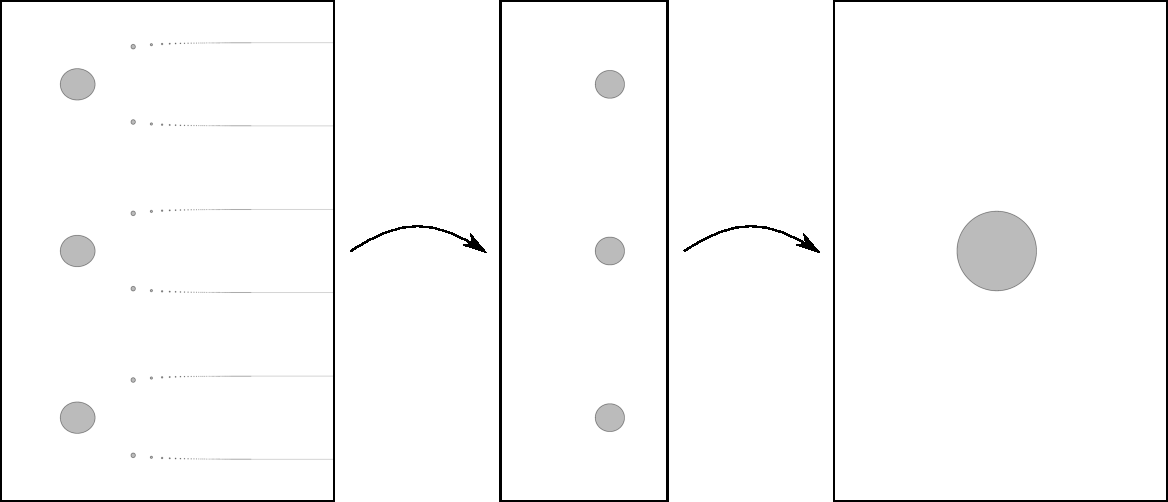
\includegraphics[width=0.6\textwidth]{preimages.pdf}
        \caption[]{Ilustracija dokaza leme \ref{lem:inversebranches}. Prikazani sta prva in druga praslika komponente za povezanost diska \(\triangle = D_{\frac{3}{2}} (3)\).}
        \label{fig:preimages}
    \end{figure}

    Bolj natančno, naj bodo \(w_n \coloneq L_n (z_0) \in V_n\). Naj bo \(\rho_1 \coloneq |w_0| + 3\) in naj bo \(D\) disk s polmerom \(2 \pi\) in sredičem v točki \(\zeta\), tako da je \(\re \zeta \geq \rho_1\). Ker je \(w_n = w_0 + n \cdot 2 \pi i\), obstaja \(n_0 \geq 1\), tako da
    \begin{equation} \label{eqn:zest}
        \abs{e^{\zeta}} - \pi \leq \abs{w_{n_0}} \leq \abs{e^{\zeta}} + \pi.
    \end{equation}
    Naj bo \(m\) tak, da je \(|\im \zeta - (4 m + 1) \pi / 2| \leq \pi\) in naj bo \(\psi\) veja logaritma, ki zgornjo polravnino preslika v pas \(\set{z \in \CC : 2 m \pi < \im z < (2 m + 1) \pi}\).

    Naj bo \(w \in V_{n_0}\). Potem velja \(|\im \psi (w) - \im \zeta| \leq 3 \pi / 2\) po definiciji \(\psi\). Še več, po definiciji \(\triangle\) in \(L_n\) velja
    \[\abs{\re w - \re w_{n_0}} = \abs{\log \frac{|e^w|}{|z_0|}} \leq \log 2.\]
    Po enačbi \eqref{eqn:zest} zaključimo, da
    \[\abs{e^{\zeta}} - 2 \pi - \log 2 \leq |w| \leq \abs{e^{\zeta}} + 2 \pi + \log 2.\]
    Delimo z \(|e^{\zeta}|\) in upoštevajoč \(\re \zeta \geq \rho_1 > 3 > \log 5 \pi\) vidimo
    \[\frac{1}{2} < 1 - \frac{2 \pi + \log 2}{|e^{\zeta}|} < \frac{|w|}{|e^{\zeta}|} < 1 + \frac{2 \pi + \log 2}{|e^{\zeta}|} < 2.\]
    Torej
    \[\abs{\re \psi (w) - \re \zeta} = \abs{\log |w| - \re \zeta} = \abs{\log \frac{|w|}{|e^{\zeta}|}} < \log 2.\]
    Zato
    \[|\psi (w) - \zeta| < \frac{3 \pi}{2} + \log 2 < 2 \pi,\]
    in zato \(\psi (V_n) \subset D\). Torej veja \(\phi \coloneq \psi \circ \varphi_n\) res preslika \(\triangle\) v \(D\). Dodatno za vsak \(z \in \triangle\) velja
    \[\phi_{n}' (z) = \frac{1}{|z|} \leq \frac{2}{|z_0|}\]
    in za vsak \(z \in V_n\):
    \[|\psi' (z)| = \frac{1}{|w|} \leq \frac{2}{e^{\zeta}}.\]
    Torej za \(\rho \coloneq \max \set{\rho_1, \log 4 - \log |z_0|}\) velja \(|\phi' (z)| \leq 1\) za vsak \(z \in \triangle\).
\end{dokaz}

\begin{dokaz}[Dokaz izreka \ref{thm:periodicdense}]
    Naj bo \(U \subset \CC\) odprta in neprazna množica. Po izreku \ref{thm:escapingdense} obstaja ubežna točka \(z_0 \in U \setminus \set{0}\). Naj bo \(\triangle\) disk s središčem v \(z_0\) in \(\rho > 0\) kot v lemi \ref{lem:inversebranches}. Disku \(\triangle\) zmanjšamo polmer, da velja \(\triangle \subset U\).

    Naj bo \(\triangle_1\) disk s središčem v \(z_0\), tako da velja \(\overline{\triangle_1} \subset \triangle\). Naj bodo \(z_n \coloneq f^n (z_0)\) in \(D_n \coloneq D_{2 \pi} (z_n)\) kot v razdelku \ref{sec:transitivity}. Naj bodo \(\set{\phi_n}_{n \geq n_0}\) inverzne veje iz trditve \ref{prop:small_disks}. Po točkah \ref{item:tri} in \ref{item:stiri} iz te trditve vemo, da je \(n_0\) dovolj velik, da velja \(\phi_n (z) \in \triangle_1\) in \(|\phi_n' (z)| \leq 1 / 2\) za vsak \(z \in D_n\).

    Ker je \(z_0\) ubežna, obsataja \(N \geq n_0\) z \(\re z_n \geq \rho\) za vsak \(n \geq N\). Šp lemi \ref{lem:inversebranches} imamo vejo \(\psi_n\) preslikave \(f^{-2}\) ki preslika \(\triangle\) v \(D_n\), za katero za vsak \(z \in \triangle\) velja \(|\psi_n' (z)| \leq 1\).
    
    Sledi \(\phi_n (\psi_n (\overline{\triangle_1}))\) in da je \(\phi_n \circ \psi_{n} \colon \overline{\triangle_1} \to \overline{\triangle_1}\) skrčitev. Ker je \(\overline{\triangle_1}\) kompaktna množica in zato poln podprostor prostora \(\CC\), lahko uporabimo Banachovo skrčitveno načelo, ki nam pove, da obstaja fiksna točka \(p \in \overline{\triangle}\). Po konstrukciji
    \begin{align*}
        f^{n + 2} (p) &= f^2 (f^n (\phi_n (\psi_n (p)))) = f^2 (\psi_n (p)) = p\\
        \intertext{in}
        |(f^{n + 2})' (p)| &= \frac{1}{|\psi_n' (p)| \cdot |\phi_n' (\psi_n (p))|} \geq 2.
    \end{align*}
    Torej je \(p\) res odbojna periodična točka \(f\).
\end{dokaz}